
\chapter{Related Literature and Studies}
\begin{refsection}

The process of data collection began with analysis of the physical principles underlying optical light emission. For illustration purposes, see \ref{fig:secondFig}.

\section{Review of Related Literature and Studies}


Depending on the energy of a photon, it may be referred to as ``light'' (in the case of optical photons) or as something else -- for example, a gamma ray. By convention, there are many names for these particles \citeauthor{allen2019fast} [\citeyear{allen2019fast}].

\subsection{Low-energy photons}

The lowest energy electromagnetic radiation is carried by radio waves.

\subsection{Intermediate-energy photons}

These include several types of radiation, including the usually-harmful.

\subsubsection{Microwaves}

Microwaves have wavelengths on the order of \SI{1e-2}{\meter}, or a few \si{\centi\meter}.

\subsubsection{Visible light}

Visible light is that which is detectable by the human eye, with wavelengths about \SIrange{380}{750}{\nano\meter}.

\begin{rotatepage}
\begin{sidewaysfigure}[!t]
    \centering
    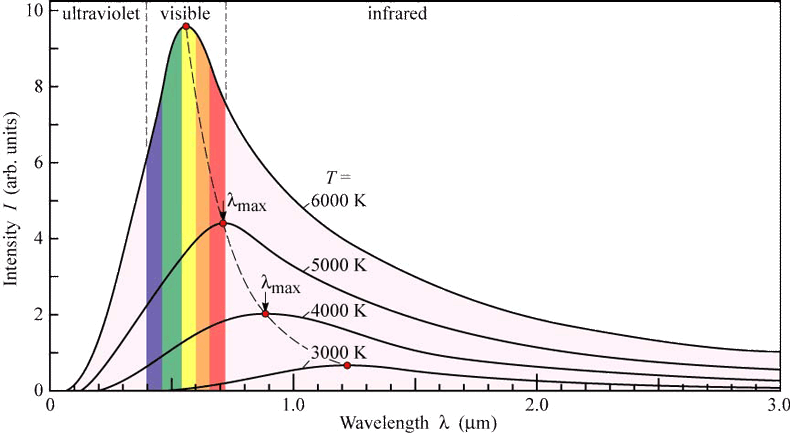
\includegraphics[width=\textwidth]{figures/sampleFig2.png}
    \caption[Black-body radiation ddd dddd dddd]{Spectra of black-body radiation at various temperatures, according to Wien's displacement law \cite{wannier1987statistical}.}
    \label{fig:secondFig}
\end{sidewaysfigure}
\end{rotatepage}

\begin{figure}[ht]
    \centering
	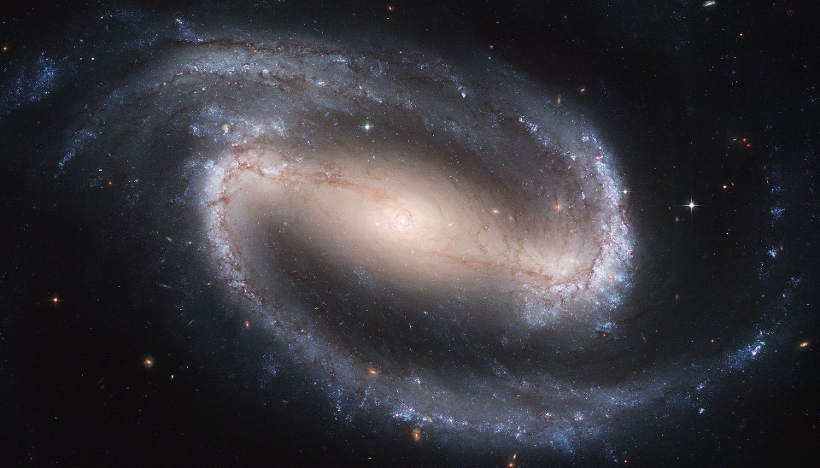
\includegraphics[width=0.85\textwidth]{figures/sampleFig1.jpg} 
	\caption[Barred spiral galaxy NGC 1300]{Barred spiral galaxy NGC 1300 photographed by Hubble telescope. While the galaxy in the photo is not our sun, it does emit light, much like our sun. Image credit: NASA.}
	\label{fig:firstFig}
\end{figure}



%=======================================================%
%%%%% Do not delete this part %%%%%%
\clearpage

\printbibliography[heading=subbibintoc, title={\texorpdfstring{\centering}{} Notes}]
\end{refsection}